\clearpage
\appendix % Optional: Setzt Nummerierung auf A, B, C...
\section{Messergebnisse}
\label{chap:anhang_content}

In diesem Anhang sind die detaillierten Messwerttabellen der durchgeführten Untersuchungen aufgeführt.

\begin{table}[H]
    \centering
    \setlength{\tabcolsep}{4pt}
    \caption{Messergebnisse: Redur 13A1030.3ffp, 2000\,A, 8,1\,$\Omega$}
    \label{tab:messergebnisse_redur_2000A}
    \small
    \begin{tabular}{
            l
            c
            S[table-format=1.3]
            S[table-format=1.2]
            S[table-format=1.3]
            S[table-format=1.2]
            S[table-format=-1.3]
            S[table-format=1.2]
            S[table-format=-1.3]
            S[table-format=2.2]
        }
        \toprule
        {}          & {}    & \multicolumn{2}{c}{5\,\% $I_n$} & \multicolumn{2}{c}{20\,\% $I_n$} & \multicolumn{2}{c}{100\,\% $I_n$} & \multicolumn{2}{c}{120\,\% $I_n$}                                   \\
        {}          & {}    & \multicolumn{2}{c}{(100\,A)}    & \multicolumn{2}{c}{(400\,A)}     & \multicolumn{2}{c}{(2000\,A)}     & \multicolumn{2}{c}{(2400\,A)}                                       \\
        \cmidrule(lr){3-4} \cmidrule(lr){5-6} \cmidrule(lr){7-8} \cmidrule(lr){9-10}
        {Geometrie} & {Ph.} & {[\%]}                          & {[A]}                            & {[\%]}                            & {[A]}                             & {[\%]} & {[A]} & {[\%]} & {[A]} \\
        \midrule
        Dreieck     & L1    & 0.473                           & 0.47                             & 0.022                             & 0.09                              & -0.120 & 2.40  & -0.121 & 2.90  \\
        Dreieck     & L2    & 0.338                           & 0.34                             & 0.088                             & 0.35                              & -0.094 & 1.88  & -1.533 & 36.79 \\
        Dreieck     & L3    & 0.471                           & 0.47                             & 0.111                             & 0.44                              & 0.126  & 2.52  & -0.070 & 1.68  \\
        \addlinespace
        Parallel    & L1    & 0.376                           & 0.38                             & 0.058                             & 0.23                              & -0.081 & 1.62  & -0.103 & 2.47  \\
        Parallel    & L2    & 0.445                           & 0.45                             & 0.111                             & 0.44                              & -0.029 & 0.58  & -0.509 & 12.22 \\
        Parallel    & L3    & 0.405                           & 0.41                             & 0.146                             & 0.58                              & 0.017  & 0.34  & -0.007 & 0.17  \\
        \bottomrule
    \end{tabular}
\end{table}

\begin{table}[H]
    \centering
    \setlength{\tabcolsep}{4pt}
    \caption{Messergebnisse: Celsa ALO 10030, 2000\,A, 1,35\,$\Omega$}
    \label{tab:messergebnisse_celsa_2000A}
    \small
    \begin{tabular}{
            l
            c
            S[table-format=1.3]
            S[table-format=1.2]
            S[table-format=-1.3]
            S[table-format=1.2]
            S[table-format=-1.3]
            S[table-format=2.2]
            S[table-format=-1.3]
            S[table-format=3.2]
        }
        \toprule
        {}          & {}    & \multicolumn{2}{c}{5\,\% $I_n$} & \multicolumn{2}{c}{20\,\% $I_n$} & \multicolumn{2}{c}{100\,\% $I_n$} & \multicolumn{2}{c}{120\,\% $I_n$}                                    \\
        {}          & {}    & \multicolumn{2}{c}{(100\,A)}    & \multicolumn{2}{c}{(400\,A)}     & \multicolumn{2}{c}{(2000\,A)}     & \multicolumn{2}{c}{(2400\,A)}                                        \\
        \cmidrule(lr){3-4} \cmidrule(lr){5-6} \cmidrule(lr){7-8} \cmidrule(lr){9-10}
        {Geometrie} & {Ph.} & {[\%]}                          & {[A]}                            & {[\%]}                            & {[A]}                             & {[\%]} & {[A]} & {[\%]} & {[A]}  \\
        \midrule
        Dreieck     & L1    & 0.183                           & 0.18                             & -0.103                            & 0.41                              & -0.273 & 5.46  & -0.317 & 7.61   \\
        Dreieck     & L2    & 0.530                           & 0.53                             & -0.026                            & 0.10                              & -0.211 & 4.22  & -0.230 & 5.52   \\
        Dreieck     & L3    & 0.480                           & 0.48                             & 0.072                             & 0.29                              & -0.153 & 3.06  & -0.758 & 18.19  \\
        \addlinespace
        Parallel    & L1    & 0.196                           & 0.20                             & -0.068                            & 0.27                              & -0.477 & 9.54  & -2.671 & 64.10  \\
        Parallel    & L2    & 0.201                           & 0.20                             & -0.014                            & 0.06                              & -1.971 & 39.42 & -4.240 & 101.76 \\
        Parallel    & L3    & 0.401                           & 0.40                             & 0.083                             & 0.33                              & -0.427 & 8.54  & -3.071 & 73.70  \\
        \bottomrule
    \end{tabular}
\end{table}

\begin{table}[H]
    \centering
    \setlength{\tabcolsep}{4pt}
    \caption{Messergebnisse: Celsa ALO 8030 K, 2000\,A, 8,1\,$\Omega$}
    \label{tab:messergebnisse_celsa8030_2000A}
    \small
    \begin{tabular}{
            l
            c
            S[table-format=1.3]
            S[table-format=1.2]
            S[table-format=-1.3]
            S[table-format=1.2]
            S[table-format=-1.3]
            S[table-format=1.2]
            S[table-format=-1.3]
            S[table-format=2.2]
        }
        \toprule
        {}          & {}    & \multicolumn{2}{c}{5\,\% $I_n$} & \multicolumn{2}{c}{20\,\% $I_n$} & \multicolumn{2}{c}{100\,\% $I_n$} & \multicolumn{2}{c}{120\,\% $I_n$}                                   \\
        {}          & {}    & \multicolumn{2}{c}{(100\,A)}    & \multicolumn{2}{c}{(400\,A)}     & \multicolumn{2}{c}{(2000\,A)}     & \multicolumn{2}{c}{(2400\,A)}                                       \\
        \cmidrule(lr){3-4} \cmidrule(lr){5-6} \cmidrule(lr){7-8} \cmidrule(lr){9-10}
        {Geometrie} & {Ph.} & {[\%]}                          & {[A]}                            & {[\%]}                            & {[A]}                             & {[\%]} & {[A]} & {[\%]} & {[A]} \\
        \midrule
        Dreieck     & L1    & 0.114                           & 0.11                             & -0.115                            & 0.46                              & -0.306 & 6.12  & -0.338 & 8.11  \\
        Dreieck     & L2    & 0.220                           & 0.22                             & -0.134                            & 0.54                              & -0.279 & 5.58  & -0.299 & 7.18  \\
        Dreieck     & L3    & 0.232                           & 0.23                             & -0.110                            & 0.44                              & -0.252 & 5.04  & -0.295 & 7.08  \\
        \addlinespace
        Parallel    & L1    & 0.134                           & 0.13                             & -0.222                            & 0.89                              & -0.354 & 7.08  & -0.428 & 10.27 \\
        Parallel    & L2    & 0.091                           & 0.09                             & -0.135                            & 0.54                              & -0.268 & 5.36  & -0.354 & 8.50  \\
        Parallel    & L3    & 0.211                           & 0.21                             & -0.055                            & 0.22                              & -0.200 & 4.00  & -0.217 & 5.21  \\
        \bottomrule
    \end{tabular}
\end{table}

\begin{table}[H]
    \centering
    \setlength{\tabcolsep}{4pt}
    \caption{Messergebnisse: MBS ASK101.4, 2000\,A, 8,1\,$\Omega$}
    \label{tab:messergebnisse_mbs_2000A}
    \small
    \begin{tabular}{
            l
            c
            S[table-format=1.3]
            S[table-format=1.2]
            S[table-format=-1.3]
            S[table-format=1.2]
            S[table-format=-1.3]
            S[table-format=1.2]
            S[table-format=-1.3]
            S[table-format=2.2]
        }
        \toprule
        {}          & {}    & \multicolumn{2}{c}{5\,\% $I_n$} & \multicolumn{2}{c}{20\,\% $I_n$} & \multicolumn{2}{c}{100\,\% $I_n$} & \multicolumn{2}{c}{120\,\% $I_n$}                                   \\
        {}          & {}    & \multicolumn{2}{c}{(100\,A)}    & \multicolumn{2}{c}{(400\,A)}     & \multicolumn{2}{c}{(2000\,A)}     & \multicolumn{2}{c}{(2400\,A)}                                       \\
        \cmidrule(lr){3-4} \cmidrule(lr){5-6} \cmidrule(lr){7-8} \cmidrule(lr){9-10}
        {Geometrie} & {Ph.} & {[\%]}                          & {[A]}                            & {[\%]}                            & {[A]}                             & {[\%]} & {[A]} & {[\%]} & {[A]} \\
        \midrule
        Dreieck     & L1    & 0.133                           & 0.13                             & -0.097                            & 0.39                              & -0.284 & 5.68  & -0.305 & 7.32  \\
        Dreieck     & L2    & -0.279                          & 0.28                             & -0.248                            & 0.99                              & -0.204 & 4.08  & -0.232 & 5.57  \\
        Dreieck     & L3    & 0.016                           & 0.02                             & -0.044                            & 0.18                              & -0.163 & 3.26  & -0.166 & 3.98  \\
        \addlinespace
        Parallel    & L1    & 0.134                           & 0.13                             & -0.222                            & 0.89                              & -0.353 & 7.06  & -0.428 & 10.27 \\
        Parallel    & L2    & 0.091                           & 0.09                             & -0.135                            & 0.54                              & -0.268 & 5.36  & -0.355 & 8.52  \\
        Parallel    & L3    & 0.211                           & 0.21                             & -0.056                            & 0.22                              & -0.200 & 4.00  & -0.217 & 5.21  \\
        \bottomrule
    \end{tabular}
\end{table}

\begin{table}[H]
    \centering
    \caption{Gesamtmessergebnisse: Celsa ALO 10050 K, 2500\,A, 2,8\,$\Omega$ (Alle Lastpunkte)}
    \label{tab:messergebnisse_celsa10050_2500A_alle}
    \setlength{\tabcolsep}{2pt}
    \scriptsize
    \resizebox{\textwidth}{!}{%
        \begin{tabular}{
                l
                c
                S[table-format=-1.3] S[table-format=1.2]
                S[table-format=-1.3] S[table-format=1.2]
                S[table-format=-1.3] S[table-format=1.2]
                S[table-format=-1.3] S[table-format=1.2]
                S[table-format=-1.3] S[table-format=1.2]
                S[table-format=-1.3] S[table-format=1.2]
                S[table-format=-1.3] S[table-format=2.2]
            }
            \toprule
            {}       & {}    & \multicolumn{2}{c}{5\,\%}    & \multicolumn{2}{c}{20\,\%}   & \multicolumn{2}{c}{50\,\%}    & \multicolumn{2}{c}{80\,\%}    & \multicolumn{2}{c}{90\,\%}    & \multicolumn{2}{c}{100\,\%}   & \multicolumn{2}{c}{120\,\%}                                                              \\
            {}       & {}    & \multicolumn{2}{c}{(125\,A)} & \multicolumn{2}{c}{(500\,A)} & \multicolumn{2}{c}{(1250\,A)} & \multicolumn{2}{c}{(2000\,A)} & \multicolumn{2}{c}{(2250\,A)} & \multicolumn{2}{c}{(2500\,A)} & \multicolumn{2}{c}{(3000\,A)}                                                            \\
            \cmidrule(lr){3-4} \cmidrule(lr){5-6} \cmidrule(lr){7-8} \cmidrule(lr){9-10} \cmidrule(lr){11-12} \cmidrule(lr){13-14} \cmidrule(lr){15-16}
            {Geom.}  & {Ph.} & {[\%]}                       & {[A]}                        & {[\%]}                        & {[A]}                         & {[\%]}                        & {[A]}                         & {[\%]}                        & {[A]} & {[\%]} & {[A]} & {[\%]} & {[A]} & {[\%]} & {[A]} \\
            \midrule
            Dreieck  & L1    & -0.029                       & 0.04                         & -0.186                        & 0.93                          & -0.229                        & 2.86                          & -0.255                        & 5.10  & -0.259 & 5.83  & -0.279 & 6.97  & -0.305 & 9.16  \\
            Dreieck  & L2    & 0.009                        & 0.01                         & -0.140                        & 0.70                          & -0.188                        & 2.35                          & -0.222                        & 4.44  & -0.242 & 5.44  & -0.275 & 6.87  & -0.549 & 16.47 \\
            Dreieck  & L3    & 0.102                        & 0.13                         & -0.077                        & 0.38                          & -0.126                        & 1.57                          & -0.171                        & 3.42  & -0.192 & 4.33  & -0.229 & 5.72  & -0.317 & 9.52  \\
            \addlinespace
            Parallel & L1    & 0.081                        & 0.10                         & -0.164                        & 0.82                          & -0.232                        & 2.90                          & -0.273                        & 5.45  & -0.306 & 6.89  & -0.291 & 7.28  & -0.326 & 9.77  \\
            Parallel & L2    & 0.247                        & 0.31                         & -0.104                        & 0.52                          & -0.192                        & 2.40                          & -0.238                        & 4.76  & -0.301 & 6.78  & -0.372 & 9.31  & -1.012 & 30.35 \\
            Parallel & L3    & 0.234                        & 0.29                         & -0.053                        & 0.27                          & -0.135                        & 1.68                          & -0.173                        & 3.45  & -0.199 & 4.49  & -0.197 & 4.93  & -0.264 & 7.92  \\
            \bottomrule
        \end{tabular}
    }
\end{table}

\begin{table}[H]
    \centering
    \caption{Gesamtmessergebnisse: Celsa ALO 10030, 2500\,A, 1,35\,$\Omega$ (Alle Lastpunkte)}
    \label{tab:messergebnisse_celsa10030_2500A_alle}
    \setlength{\tabcolsep}{2pt} % Sehr kleiner Spaltenabstand
    \scriptsize % Sehr kleine Schrift
    \resizebox{\textwidth}{!}{% Skaliert die Tabelle auf Textbreite
        \begin{tabular}{
                l
                c
                S[table-format=1.3] S[table-format=1.2]
                S[table-format=-1.3] S[table-format=1.2]
                S[table-format=-1.3] S[table-format=2.2]
                S[table-format=-2.3] S[table-format=3.2]
                S[table-format=-2.3] S[table-format=3.2]
                S[table-format=-2.3] S[table-format=3.2]
                S[table-format=-2.3] S[table-format=3.2]
            }
            \toprule
            {}       & {}    & \multicolumn{2}{c}{5\,\%}    & \multicolumn{2}{c}{20\,\%}   & \multicolumn{2}{c}{50\,\%}    & \multicolumn{2}{c}{80\,\%}    & \multicolumn{2}{c}{90\,\%}    & \multicolumn{2}{c}{100\,\%}   & \multicolumn{2}{c}{120\,\%}                                                                     \\
            {}       & {}    & \multicolumn{2}{c}{(125\,A)} & \multicolumn{2}{c}{(500\,A)} & \multicolumn{2}{c}{(1250\,A)} & \multicolumn{2}{c}{(2000\,A)} & \multicolumn{2}{c}{(2250\,A)} & \multicolumn{2}{c}{(2500\,A)} & \multicolumn{2}{c}{(3000\,A)}                                                                   \\
            \cmidrule(lr){3-4} \cmidrule(lr){5-6} \cmidrule(lr){7-8} \cmidrule(lr){9-10} \cmidrule(lr){11-12} \cmidrule(lr){13-14} \cmidrule(lr){15-16}
            {Geom.}  & {Ph.} & {[\%]}                       & {[A]}                        & {[\%]}                        & {[A]}                         & {[\%]}                        & {[A]}                         & {[\%]}                        & {[A]}  & {[\%]}  & {[A]}  & {[\%]}  & {[A]}  & {[\%]}  & {[A]}  \\
            \midrule
            Dreieck  & L1    & 0.159                        & 0.20                         & -0.107                        & 0.53                          & -0.247                        & 3.09                          & -1.678                        & 33.56  & -3.337  & 75.08  & -5.066  & 126.65 & -8.278  & 248.33 \\
            Dreieck  & L2    & 0.073                        & 0.09                         & -0.204                        & 1.02                          & -0.316                        & 3.95                          & -1.568                        & 31.35  & -1.763  & 39.67  & -1.834  & 45.85  & -1.950  & 58.49  \\
            Dreieck  & L3    & 0.182                        & 0.23                         & -0.139                        & 0.69                          & -0.256                        & 3.20                          & -1.126                        & 22.53  & -2.232  & 50.22  & -3.452  & 86.29  & -5.437  & 163.12 \\
            \addlinespace
            Parallel & L1    & -0.061                       & 0.08                         & -0.214                        & 1.07                          & -0.653                        & 8.17                          & -7.423                        & 148.46 & -10.056 & 226.26 & -12.370 & 309.25 & -16.238 & 487.15 \\
            Parallel & L2    & 0.060                        & 0.08                         & -0.117                        & 0.59                          & -2.732                        & 34.15                         & -11.571                       & 231.42 & -14.277 & 321.22 & -16.623 & 415.59 & -20.565 & 616.96 \\
            Parallel & L3    & 0.180                        & 0.23                         & 0.031                         & 0.16                          & -0.119                        & 1.48                          & -5.352                        & 107.03 & -7.856  & 176.77 & -10.099 & 252.46 & -13.862 & 415.87 \\
            \bottomrule
        \end{tabular}
    }
\end{table}


\begin{table}[H]
    \centering
    \caption{Gesamtmessergebnisse Celsa ALO 12070 bei 3000\,A und 10,8\,$\Omega$ (Alle Lastpunkte)}
    \label{tab:messergebnisse_celsa12070_3000A_alle}
    \setlength{\tabcolsep}{2pt}
    \scriptsize
    \resizebox{\textwidth}{!}{%
        \begin{tabular}{
                l
                c
                S[table-format=1.3] S[table-format=1.2]
                S[table-format=-1.3] S[table-format=1.2]
                S[table-format=-1.3] S[table-format=1.2]
                S[table-format=-1.3] S[table-format=2.2]
                S[table-format=-1.3] S[table-format=2.2]
                S[table-format=-1.3] S[table-format=2.2]
                S[table-format=-1.3] S[table-format=3.2]
            }
            \toprule
            {}       & {}    & \multicolumn{2}{c}{5\,\%}    & \multicolumn{2}{c}{20\,\%}   & \multicolumn{2}{c}{50\,\%}    & \multicolumn{2}{c}{80\,\%}    & \multicolumn{2}{c}{90\,\%}    & \multicolumn{2}{c}{100\,\%}   & \multicolumn{2}{c}{120\,\%}                                                               \\
            {}       & {}    & \multicolumn{2}{c}{(150\,A)} & \multicolumn{2}{c}{(600\,A)} & \multicolumn{2}{c}{(1500\,A)} & \multicolumn{2}{c}{(2400\,A)} & \multicolumn{2}{c}{(2700\,A)} & \multicolumn{2}{c}{(3000\,A)} & \multicolumn{2}{c}{(3600\,A)}                                                             \\
            \cmidrule(lr){3-4} \cmidrule(lr){5-6} \cmidrule(lr){7-8} \cmidrule(lr){9-10} \cmidrule(lr){11-12} \cmidrule(lr){13-14} \cmidrule(lr){15-16}
            {Geom.}  & {Ph.} & {[\%]}                       & {[A]}                        & {[\%]}                        & {[A]}                         & {[\%]}                        & {[A]}                         & {[\%]}                        & {[A]} & {[\%]} & {[A]} & {[\%]} & {[A]} & {[\%]} & {[A]}  \\
            \midrule
            Dreieck  & L1    & 0.138                        & 0.21                         & -0.174                        & 1.04                          & -0.257                        & 3.86                          & -0.314                        & 7.53  & -0.343 & 9.26  & -0.385 & 11.54 & -0.685 & 24.64  \\
            Dreieck  & L2    & 0.201                        & 0.30                         & -0.093                        & 0.56                          & -0.173                        & 2.60                          & -0.196                        & 4.69  & -0.201 & 5.43  & -0.207 & 6.20  & -0.227 & 8.16   \\
            Dreieck  & L3    & 0.330                        & 0.50                         & 0.059                         & 0.36                          & -0.050                        & 0.75                          & -0.113                        & 2.71  & -0.136 & 3.67  & -0.035 & 1.05  & -0.018 & 0.65   \\
            \addlinespace
            Parallel & L1    & 0.265                        & 0.40                         & -0.195                        & 1.17                          & -0.225                        & 3.38                          & -0.301                        & 7.22  & -0.349 & 9.43  & -0.418 & 12.53 & -1.017 & 36.63  \\
            Parallel & L2    & 0.285                        & 0.43                         & -0.089                        & 0.54                          & -0.158                        & 2.37                          & -1.081                        & 25.94 & -1.890 & 51.02 & -2.924 & 87.73 & -5.426 & 195.33 \\
            Parallel & L3    & 0.253                        & 0.38                         & -0.030                        & 0.18                          & -0.098                        & 1.47                          & -0.138                        & 3.31  & -0.149 & 4.02  & -0.170 & 5.10  & -0.910 & 32.77  \\
            \bottomrule
        \end{tabular}
    }
\end{table}

\begin{table}[H]
    \centering
    \caption{Gesamtmessergebnisse Celsa ALO 12070 K bei 3000\,A und 10,8\,$\Omega$ (Alle Lastpunkte)}
    \label{tab:messergebnisse_celsa12070K_3000A_alle}
    \setlength{\tabcolsep}{2pt}
    \scriptsize
    \resizebox{\textwidth}{!}{%
        \begin{tabular}{
                l
                c
                S[table-format=1.3] S[table-format=1.2]
                S[table-format=-1.3] S[table-format=1.2]
                S[table-format=-1.3] S[table-format=1.2]
                S[table-format=-1.3] S[table-format=1.2]
                S[table-format=-1.3] S[table-format=1.2]
                S[table-format=-1.3] S[table-format=1.2]
                S[table-format=-1.3] S[table-format=2.2]
            }
            \toprule
            {}       & {}    & \multicolumn{2}{c}{5\,\%}    & \multicolumn{2}{c}{20\,\%}   & \multicolumn{2}{c}{50\,\%}    & \multicolumn{2}{c}{80\,\%}    & \multicolumn{2}{c}{90\,\%}    & \multicolumn{2}{c}{100\,\%}   & \multicolumn{2}{c}{120\,\%}                                                              \\
            {}       & {}    & \multicolumn{2}{c}{(150\,A)} & \multicolumn{2}{c}{(600\,A)} & \multicolumn{2}{c}{(1500\,A)} & \multicolumn{2}{c}{(2400\,A)} & \multicolumn{2}{c}{(2700\,A)} & \multicolumn{2}{c}{(3000\,A)} & \multicolumn{2}{c}{(3600\,A)}                                                            \\
            \cmidrule(lr){3-4} \cmidrule(lr){5-6} \cmidrule(lr){7-8} \cmidrule(lr){9-10} \cmidrule(lr){11-12} \cmidrule(lr){13-14} \cmidrule(lr){15-16}
            {Geom.}  & {Ph.} & {[\%]}                       & {[A]}                        & {[\%]}                        & {[A]}                         & {[\%]}                        & {[A]}                         & {[\%]}                        & {[A]} & {[\%]} & {[A]} & {[\%]} & {[A]} & {[\%]} & {[A]} \\
            \midrule
            Dreieck  & L1    & 0.273                        & 0.41                         & -0.093                        & 0.56                          & -0.170                        & 2.54                          & -0.184                        & 4.43  & -0.163 & 4.41  & -0.141 & 4.23  & -0.076 & 2.75  \\
            Dreieck  & L2    & 0.296                        & 0.44                         & 0.022                         & 0.13                          & -0.073                        & 1.10                          & -0.108                        & 2.58  & -0.088 & 2.38  & -0.073 & 2.20  & 0.097  & 3.48  \\
            Dreieck  & L3    & 0.338                        & 0.51                         & 0.153                         & 0.92                          & 0.137                         & 2.05                          & 0.169                         & 4.06  & -0.037 & 1.01  & -0.045 & 1.35  & -0.046 & 1.65  \\
            \addlinespace
            Parallel & L1    & 0.194                        & 0.29                         & -0.070                        & 0.42                          & -0.176                        & 2.64                          & -0.174                        & 4.18  & -0.150 & 4.05  & -0.118 & 3.55  & -0.072 & 2.59  \\
            Parallel & L2    & 0.209                        & 0.31                         & -0.009                        & 0.05                          & -0.099                        & 1.48                          & -0.071                        & 1.70  & 0.022  & 0.58  & 0.266  & 7.98  & 0.929  & 33.44 \\
            Parallel & L3    & 0.345                        & 0.52                         & 0.110                         & 0.66                          & 0.001                         & 0.01                          & -0.031                        & 0.73  & -0.018 & 0.50  & 0.012  & 0.37  & 0.082  & 2.95  \\
            \bottomrule
        \end{tabular}
    }
\end{table}

\begin{table}[H]
    \centering
    \caption{Messergebnisse: Celsa ALO 12070, 3000\,A, Asymmetrische Bürde ($R_{L2} = 0\,\Omega$, Parallel)}
    \label{tab:messergebnisse_celsa12070_3000A_asym}
    \setlength{\tabcolsep}{2pt}
    \scriptsize
    \resizebox{\textwidth}{!}{%
        \begin{tabular}{
                l
                c
                S[table-format=1.3] S[table-format=1.2]
                S[table-format=-1.3] S[table-format=1.2]
                S[table-format=-1.3] S[table-format=1.2]
                S[table-format=-1.3] S[table-format=2.2]
                S[table-format=-1.3] S[table-format=2.2]
                S[table-format=-1.3] S[table-format=2.2]
                S[table-format=-1.3] S[table-format=3.2]
            }
            \toprule
            {}       & {}    & \multicolumn{2}{c}{5\,\%}    & \multicolumn{2}{c}{20\,\%}   & \multicolumn{2}{c}{50\,\%}    & \multicolumn{2}{c}{80\,\%}    & \multicolumn{2}{c}{90\,\%}    & \multicolumn{2}{c}{100\,\%}   & \multicolumn{2}{c}{120\,\%}                                                                     \\
            {}       & {}    & \multicolumn{2}{c}{(150\,A)} & \multicolumn{2}{c}{(600\,A)} & \multicolumn{2}{c}{(1500\,A)} & \multicolumn{2}{c}{(2400\,A)} & \multicolumn{2}{c}{(2700\,A)} & \multicolumn{2}{c}{(3000\,A)} & \multicolumn{2}{c}{(3600\,A)}                                                                   \\
            \cmidrule(lr){3-4} \cmidrule(lr){5-6} \cmidrule(lr){7-8} \cmidrule(lr){9-10} \cmidrule(lr){11-12} \cmidrule(lr){13-14} \cmidrule(lr){15-16}
            {Geom.}  & {Ph.} & {[\%]}                       & {[A]}                        & {[\%]}                        & {[A]}                         & {[\%]}                        & {[A]}                         & {[\%]}                        & {[A]}  & {[\%]}  & {[A]}  & {[\%]}  & {[A]}  & {[\%]}  & {[A]}   \\
            \midrule
            Parallel & L1    & 0.063                        & 0.09                         & -0.157                        & 0.94                          & -0.225                        & 3.38                          & -0.306                        & 7.34   & -0.348  & 9.39   & -0.417  & 12.51  & -1.043  & 37.56   \\
            Parallel & L2    & 0.191                        & 0.29                         & -0.061                        & 0.37                          & -0.127                        & 1.91                          & -0.817                        & 19.61  & -1.805  & 48.73  & -3.044  & 91.33  & -5.683  & 204.61  \\
            Parallel & L3    & 0.271                        & 0.41                         & -0.020                        & 0.12                          & -0.107                        & 1.61                          & -0.139                        & 3.34   & -0.151  & 4.07   & -0.163  & 4.90   & -0.726  & 26.13   \\
            \bottomrule
        \end{tabular}
    }
\end{table}

\begin{table}[H]
    \centering
    \caption{Messergebnisse: Celsa ALO 12070, 3000\,A, Minimale Bürde ($R_B \approx 0\,\Omega$, Parallel)}
    \label{tab:messergebnisse_celsa12070_3000A_min}
    \setlength{\tabcolsep}{2pt}
    \scriptsize
    \resizebox{\textwidth}{!}{%
        \begin{tabular}{
                l
                c
                S[table-format=1.3] S[table-format=1.2]
                S[table-format=-1.3] S[table-format=1.2]
                S[table-format=-1.3] S[table-format=1.2]
                S[table-format=-1.3] S[table-format=2.2]
                S[table-format=-1.3] S[table-format=2.2]
                S[table-format=-1.3] S[table-format=2.2]
                S[table-format=-1.3] S[table-format=3.2]
            }
            \toprule
            {}       & {}    & \multicolumn{2}{c}{5\,\%}    & \multicolumn{2}{c}{20\,\%}   & \multicolumn{2}{c}{50\,\%}    & \multicolumn{2}{c}{80\,\%}    & \multicolumn{2}{c}{90\,\%}    & \multicolumn{2}{c}{100\,\%}   & \multicolumn{2}{c}{120\,\%}                                                                     \\
            {}       & {}    & \multicolumn{2}{c}{(150\,A)} & \multicolumn{2}{c}{(600\,A)} & \multicolumn{2}{c}{(1500\,A)} & \multicolumn{2}{c}{(2400\,A)} & \multicolumn{2}{c}{(2700\,A)} & \multicolumn{2}{c}{(3000\,A)} & \multicolumn{2}{c}{(3600\,A)}                                                                   \\
            \cmidrule(lr){3-4} \cmidrule(lr){5-6} \cmidrule(lr){7-8} \cmidrule(lr){9-10} \cmidrule(lr){11-12} \cmidrule(lr){13-14} \cmidrule(lr){15-16}
            {Geom.}  & {Ph.} & {[\%]}                       & {[A]}                        & {[\%]}                        & {[A]}                         & {[\%]}                        & {[A]}                         & {[\%]}                        & {[A]}  & {[\%]}  & {[A]}  & {[\%]}  & {[A]}  & {[\%]}  & {[A]}   \\
            \midrule
            Parallel & L1    & 0.084                        & 0.13                         & -0.132                        & 0.79                          & -0.218                        & 3.27                          & -0.276                        & 6.62   & -0.318  & 8.58   & -0.395  & 11.86  & -1.857  & 66.85   \\
            Parallel & L2    & 0.169                        & 0.25                         & -0.039                        & 0.23                          & -0.131                        & 1.96                          & -0.598                        & 14.34  & -1.415  & 38.20  & -2.537  & 76.12  & -5.113  & 184.08  \\
            Parallel & L3    & 0.300                        & 0.45                         & 0.045                         & 0.27                          & -0.046                        & 0.69                          & -0.086                        & 2.07   & -0.099  & 2.67   & -0.121  & 3.63   & -0.428  & 15.42   \\
            \bottomrule
        \end{tabular}
    }
\end{table}


\begin{table}[H]
    \centering
    \caption{Messergebnisse Celsa ALO 12070 bei 4000 A und 0,0 Ohm für alle Lastpunkte}
    \label{tab:messergebnisse_celsa12070_4000A_alle}
    \setlength{\tabcolsep}{2pt}
    \scriptsize
    \resizebox{\textwidth}{!}{%
        \begin{tabular}{
                l
                c
                S[table-format=1.3] S[table-format=3.2]
                S[table-format=-1.3] S[table-format=3.2]
                S[table-format=-1.3] S[table-format=4.2]
                S[table-format=-1.3] S[table-format=4.2]
                S[table-format=-1.3] S[table-format=4.2]
                S[table-format=-1.3] S[table-format=4.2]
                S[table-format=-1.3] S[table-format=4.2]
            }
            \toprule
            {}       & {}    & \multicolumn{2}{c}{5\,\%} & \multicolumn{2}{c}{20\,\%} & \multicolumn{2}{c}{50\,\%} & \multicolumn{2}{c}{80\,\%} & \multicolumn{2}{c}{90\,\%} & \multicolumn{2}{c}{100\,\%} & \multicolumn{2}{c}{120\,\%} \\
            {}       & {}    & \multicolumn{2}{c}{(200\,A)} & \multicolumn{2}{c}{(800\,A)} & \multicolumn{2}{c}{(2000\,A)} & \multicolumn{2}{c}{(3200\,A)} & \multicolumn{2}{c}{(3600\,A)} & \multicolumn{2}{c}{(4000\,A)} & \multicolumn{2}{c}{(4800\,A)} \\
            \cmidrule(lr){3-4} \cmidrule(lr){5-6} \cmidrule(lr){7-8} \cmidrule(lr){9-10} \cmidrule(lr){11-12} \cmidrule(lr){13-14} \cmidrule(lr){15-16}
            {Geom.}  & {Ph.} & {[\%]} & {[A]} & {[\%]} & {[A]} & {[\%]} & {[A]} & {[\%]} & {[A]} & {[\%]} & {[A]} & {[\%]} & {[A]} & {[\%]} & {[A]} \\
            \midrule
            Parallel & L1 & 0.218 & 0.44 & -0.034 & -0.27 & -0.117 & -2.34 & -0.142 & -4.55 & -0.196 & -7.06 & -0.698 & -27.93 & -3.206 & -153.87 \\
            Parallel & L2 & 0.139 & 0.28 & -0.068 & -0.54 & -0.123 & -2.46 & -0.945 & -30.23 & -2.027 & -72.97 & -3.283 & -131.33 & -5.861 & -281.35 \\
            Parallel & L3 & 0.107 & 0.21 & -0.122 & -0.98 & -0.163 & -3.25 & -0.201 & -6.42 & -0.361 & -13.00 & -1.218 & -48.72 & -3.835 & -184.08 \\
            \addlinespace
            Dreieck & L1 & 0.248 & 0.50 & -0.044 & -0.35 & -0.117 & -2.33 & -0.143 & -4.58 & -0.159 & -5.71 & -0.227 & -9.09 & -1.489 & -71.47 \\
            Dreieck & L2 & 0.146 & 0.29 & -0.094 & -0.75 & -0.132 & -2.64 & -0.149 & -4.76 & -0.143 & -5.14 & -0.151 & -6.06 & 0.291 & 13.97 \\
            Dreieck & L3 & 0.075 & 0.15 & -0.109 & -0.87 & -0.174 & -3.48 & -0.190 & -6.08 & -0.208 & -7.48 & -0.302 & -12.08 & -1.713 & -82.20 \\
            \bottomrule
        \end{tabular}
    }
\end{table}


\begin{table}[H]
    \centering
    \caption{Messergebnisse Celsa ALO 12070 K bei 4000 A und 0,0 Ohm für alle Lastpunkte}
    \label{tab:messergebnisse_celsa12070K_4000A_alle}
    \setlength{\tabcolsep}{2pt}
    \scriptsize
    \resizebox{\textwidth}{!}{%
        \begin{tabular}{
                l
                c
                S[table-format=1.3] S[table-format=3.2]
                S[table-format=-1.3] S[table-format=3.2]
                S[table-format=-1.3] S[table-format=4.2]
                S[table-format=-1.3] S[table-format=4.2]
                S[table-format=-1.3] S[table-format=4.2]
                S[table-format=-1.3] S[table-format=4.2]
                S[table-format=-1.3] S[table-format=4.2]
            }
            \toprule
            {}       & {}    & \multicolumn{2}{c}{5\,\%} & \multicolumn{2}{c}{20\,\%} & \multicolumn{2}{c}{50\,\%} & \multicolumn{2}{c}{80\,\%} & \multicolumn{2}{c}{90\,\%} & \multicolumn{2}{c}{100\,\%} & \multicolumn{2}{c}{120\,\%} \\
            {}       & {}    & \multicolumn{2}{c}{(200\,A)} & \multicolumn{2}{c}{(800\,A)} & \multicolumn{2}{c}{(2000\,A)} & \multicolumn{2}{c}{(3200\,A)} & \multicolumn{2}{c}{(3600\,A)} & \multicolumn{2}{c}{(4000\,A)} & \multicolumn{2}{c}{(4800\,A)} \\
            \cmidrule(lr){3-4} \cmidrule(lr){5-6} \cmidrule(lr){7-8} \cmidrule(lr){9-10} \cmidrule(lr){11-12} \cmidrule(lr){13-14} \cmidrule(lr){15-16}
            {Geom.}  & {Ph.} & {[\%]} & {[A]} & {[\%]} & {[A]} & {[\%]} & {[A]} & {[\%]} & {[A]} & {[\%]} & {[A]} & {[\%]} & {[A]} & {[\%]} & {[A]} \\
            \midrule
            Parallel & L1 & 0.326 & 0.65 & 0.089 & 0.72 & 0.041 & 0.82 & 0.044 & 1.41 & 0.044 & 1.60 & 0.062 & 2.50 & 0.039 & 1.89 \\
            Parallel & L2 & 0.113 & 0.23 & -0.114 & -0.91 & -0.167 & -3.34 & -0.170 & -5.44 & -0.175 & -6.30 & -0.198 & -7.92 & -0.582 & -27.95 \\
            Parallel & L3 & 0.214 & 0.43 & 0.026 & 0.21 & -0.041 & -0.82 & -0.064 & -2.04 & -0.063 & -2.26 & -0.054 & -2.17 & -0.031 & -1.49 \\
            \addlinespace
            Dreieck & L1 & 0.424 & 0.85 & 0.117 & 0.94 & 0.050 & 1.00 & 0.041 & 1.33 & 0.039 & 1.42 & 0.057 & 2.28 & 0.076 & 3.66 \\
            Dreieck & L2 & 0.111 & 0.22 & -0.068 & -0.54 & -0.155 & -3.10 & -0.185 & -5.93 & -0.189 & -6.79 & -0.203 & -8.14 & -0.651 & -31.27 \\
            Dreieck & L3 & 0.273 & 0.55 & 0.039 & 0.32 & -0.033 & -0.66 & -0.070 & -2.23 & -0.065 & -2.36 & -0.067 & -2.67 & -0.061 & -2.92 \\
            \bottomrule
        \end{tabular}
    }
\end{table}


\begin{table}[H]
    \centering
    \caption{Messergebnisse: Celsa ALO 20060, 5000\,A, 0,0\,$\Omega$ (Alle Lastpunkte)}
    \label{tab:messergebnisse_celsa20060_5000A_alle}
    \setlength{\tabcolsep}{2pt}
    \scriptsize
    \resizebox{\textwidth}{!}{%
        \begin{tabular}{
                l
                c
                S[table-format=-1.3] S[table-format=3.2]
                S[table-format=-1.3] S[table-format=3.2]
                S[table-format=-1.3] S[table-format=3.2]
                S[table-format=-1.3] S[table-format=3.2]
                S[table-format=-1.3] S[table-format=4.2]
                S[table-format=-1.3] S[table-format=4.2]
                S[table-format=-1.3] S[table-format=4.2]
            }
            \toprule
            {}       & {}    & \multicolumn{2}{c}{5\,\%} & \multicolumn{2}{c}{20\,\%} & \multicolumn{2}{c}{50\,\%} & \multicolumn{2}{c}{80\,\%} & \multicolumn{2}{c}{90\,\%} & \multicolumn{2}{c}{100\,\%} & \multicolumn{2}{c}{120\,\%} \\
            {}       & {}    & \multicolumn{2}{c}{(250\,A)} & \multicolumn{2}{c}{(1000\,A)} & \multicolumn{2}{c}{(2500\,A)} & \multicolumn{2}{c}{(4000\,A)} & \multicolumn{2}{c}{(4500\,A)} & \multicolumn{2}{c}{(5000\,A)} & \multicolumn{2}{c}{(6000\,A)} \\
            \cmidrule(lr){3-4} \cmidrule(lr){5-6} \cmidrule(lr){7-8} \cmidrule(lr){9-10} \cmidrule(lr){11-12} \cmidrule(lr){13-14} \cmidrule(lr){15-16}
            {Geom.}  & {Ph.} & {[\%]} & {[A]} & {[\%]} & {[A]} & {[\%]} & {[A]} & {[\%]} & {[A]} & {[\%]} & {[A]} & {[\%]} & {[A]} & {[\%]} & {[A]} \\
            \midrule
            Parallel & L1 & 0.127 & 0.32 & -0.205 & -2.05 & -0.272 & -6.81 & -0.309 & -12.34 & -0.321 & -14.45 & -0.340 & -17.02 & -0.848 & -50.86 \\
            Parallel & L2 & 0.011 & 0.03 & -0.171 & -1.71 & -0.269 & -6.72 & -1.860 & -74.39 & -2.870 & -129.16 & -3.836 & -191.82 & -5.656 & -339.37 \\
            Parallel & L3 & 0.136 & 0.34 & -0.039 & -0.39 & -0.108 & -2.71 & -0.135 & -5.42 & -0.144 & -6.49 & -0.161 & -8.04 & -0.521 & -31.26 \\
            \addlinespace
            Dreieck & L1 & 0.083 & 0.21 & -0.214 & -2.14 & -0.261 & -6.53 & -0.313 & -12.50 & -0.304 & -13.69 & -0.306 & -15.29 & -0.341 & -20.43 \\
            Dreieck & L2 & 0.027 & 0.07 & -0.176 & -1.76 & -0.219 & -5.48 & -0.261 & -10.44 & -0.261 & -11.74 & -0.260 & -13.01 & -0.174 & -10.41 \\
            Dreieck & L3 & 0.198 & 0.49 & -0.035 & -0.35 & -0.103 & -2.57 & -0.137 & -5.46 & -0.140 & -6.30 & -0.146 & -7.32 & -0.176 & -10.58 \\
            \bottomrule
        \end{tabular}
    }
\end{table}


\begin{table}[H]
    \centering
    \caption{Messergebnisse: Celsa ALO E 16050 K, 5000\,A, 0,0\,$\Omega$ (Alle Lastpunkte)}
    \label{tab:messergebnisse_celsa16050K_5000A_alle}
    \setlength{\tabcolsep}{2pt}
    \scriptsize
    \resizebox{\textwidth}{!}{%
        \begin{tabular}{
                l
                c
                S[table-format=-1.3] S[table-format=3.2]
                S[table-format=-1.3] S[table-format=3.2]
                S[table-format=-1.3] S[table-format=3.2]
                S[table-format=-1.3] S[table-format=3.2]
                S[table-format=-1.3] S[table-format=4.2]
                S[table-format=-1.3] S[table-format=4.2]
                S[table-format=-1.3] S[table-format=4.2]
            }
            \toprule
            {}       & {}    & \multicolumn{2}{c}{5\,\%} & \multicolumn{2}{c}{20\,\%} & \multicolumn{2}{c}{50\,\%} & \multicolumn{2}{c}{80\,\%} & \multicolumn{2}{c}{90\,\%} & \multicolumn{2}{c}{100\,\%} & \multicolumn{2}{c}{120\,\%} \\
            {}       & {}    & \multicolumn{2}{c}{(250\,A)} & \multicolumn{2}{c}{(1000\,A)} & \multicolumn{2}{c}{(2500\,A)} & \multicolumn{2}{c}{(4000\,A)} & \multicolumn{2}{c}{(4500\,A)} & \multicolumn{2}{c}{(5000\,A)} & \multicolumn{2}{c}{(6000\,A)} \\
            \cmidrule(lr){3-4} \cmidrule(lr){5-6} \cmidrule(lr){7-8} \cmidrule(lr){9-10} \cmidrule(lr){11-12} \cmidrule(lr){13-14} \cmidrule(lr){15-16}
            {Geom.}  & {Ph.} & {[\%]} & {[A]} & {[\%]} & {[A]} & {[\%]} & {[A]} & {[\%]} & {[A]} & {[\%]} & {[A]} & {[\%]} & {[A]} & {[\%]} & {[A]} \\
            \midrule
            Parallel & L1 & 7.471 & 18.68 & 12.040 & 120.40 & 13.343 & 333.57 & 12.504 & 500.17 & 11.388 & 512.48 & 10.101 & 505.04 & 7.277 & 436.63 \\
            Parallel & L2 & 0.080 & 0.20 & -0.071 & -0.71 & -0.136 & -3.39 & -0.264 & -10.58 & -0.560 & -25.19 & -1.010 & -50.50 & -2.135 & -128.11 \\
            Parallel & L3 & 0.164 & 0.41 & -0.015 & -0.15 & -0.093 & -2.32 & -0.206 & -8.24 & -0.289 & -13.00 & -0.393 & -19.63 & -0.448 & -26.90 \\
            \addlinespace
            Dreieck & L1 & 0.131 & 0.33 & -0.078 & -0.78 & -0.152 & -3.81 & -0.189 & -7.56 & -0.210 & -9.44 & -0.221 & -11.04 & -0.596 & -35.77 \\
            Dreieck & L2 & 0.060 & 0.15 & -0.076 & -0.76 & -0.231 & -5.78 & -1.446 & -57.83 & -2.269 & -102.10 & -3.485 & -174.25 & -7.234 & -434.06 \\
            Dreieck & L3 & -3.079 & -7.70 & 0.385 & 3.85 & 0.989 & 24.73 & 0.194 & 7.75 & -0.633 & -28.48 & -1.546 & -77.31 & -3.003 & -180.20 \\
            \bottomrule
        \end{tabular}
    }
\end{table}


\begin{table}[H]
    \centering
    \caption{Messergebnisse: Redur 20A1456.5vffp, 5000\,A (Parallel 0,0\,$\Omega$, Dreieck 8,1\,$\Omega$)}
    \label{tab:messergebnisse_redur_5000A_mixed}
    \setlength{\tabcolsep}{2pt}
    \scriptsize
    \resizebox{\textwidth}{!}{%
        \begin{tabular}{
                l
                c
                S[table-format=-1.3] S[table-format=3.2]
                S[table-format=-1.3] S[table-format=3.2]
                S[table-format=-1.3] S[table-format=3.2]
                S[table-format=-1.3] S[table-format=3.2]
                S[table-format=-1.3] S[table-format=4.2]
                S[table-format=-1.3] S[table-format=4.2]
                S[table-format=-1.3] S[table-format=4.2]
            }
            \toprule
            {}       & {}    & \multicolumn{2}{c}{5\,\%} & \multicolumn{2}{c}{20\,\%} & \multicolumn{2}{c}{50\,\%} & \multicolumn{2}{c}{80\,\%} & \multicolumn{2}{c}{90\,\%} & \multicolumn{2}{c}{100\,\%} & \multicolumn{2}{c}{120\,\%} \\
            {}       & {}    & \multicolumn{2}{c}{(250\,A)} & \multicolumn{2}{c}{(1000\,A)} & \multicolumn{2}{c}{(2500\,A)} & \multicolumn{2}{c}{(4000\,A)} & \multicolumn{2}{c}{(4500\,A)} & \multicolumn{2}{c}{(5000\,A)} & \multicolumn{2}{c}{(6000\,A)} \\
            \cmidrule(lr){3-4} \cmidrule(lr){5-6} \cmidrule(lr){7-8} \cmidrule(lr){9-10} \cmidrule(lr){11-12} \cmidrule(lr){13-14} \cmidrule(lr){15-16}
            {Geom.}  & {Ph.} & {[\%]} & {[A]} & {[\%]} & {[A]} & {[\%]} & {[A]} & {[\%]} & {[A]} & {[\%]} & {[A]} & {[\%]} & {[A]} & {[\%]} & {[A]} \\
            \midrule
            Parallel & L1 & 0.041 & 0.10 & -0.215 & -2.15 & -0.262 & -6.55 & -0.372 & -14.87 & -0.871 & -39.18 & -1.851 & -92.53 & -4.265 & -255.89 \\
            Parallel & L2 & -0.097 & -0.24 & -0.204 & -2.04 & -0.346 & -8.65 & -3.242 & -129.66 & -4.429 & -199.31 & -5.476 & -273.80 & -7.054 & -423.26 \\
            Parallel & L3 & 0.080 & 0.20 & -0.084 & -0.84 & -0.137 & -3.42 & -0.158 & -6.31 & -0.175 & -7.86 & -0.214 & -10.68 & -1.100 & -66.02 \\
            \addlinespace
            Dreieck & L1 & -0.080 & -0.20 & -0.181 & -1.81 & -0.241 & -6.02 & -0.471 & -18.83 & -1.132 & -50.93 & -1.996 & -99.79 & -3.801 & -228.04 \\
            Dreieck & L2 & -0.081 & -0.20 & -0.162 & -1.62 & -0.214 & -5.35 & -0.341 & -13.63 & -0.663 & -29.83 & -1.082 & -54.08 & -1.910 & -114.61 \\
            Dreieck & L3 & -0.014 & -0.04 & -0.128 & -1.28 & -0.149 & -3.71 & -0.116 & -4.64 & -0.139 & -6.24 & -0.228 & -11.42 & -0.444 & -26.66 \\
            \bottomrule
        \end{tabular}
    }
\end{table}


\begin{table}[H]
    \centering
    \caption{Messergebnisse: MBS ASK129.10, 5000\,A, 10,8\,$\Omega$ (Dreieck)}
    \label{tab:messergebnisse_mbs_5000A_dreieck}
    \setlength{\tabcolsep}{2pt}
    \scriptsize
    \resizebox{\textwidth}{!}{%
        \begin{tabular}{
                l
                c
                S[table-format=-1.3] S[table-format=3.2]
                S[table-format=-1.3] S[table-format=3.2]
                S[table-format=-1.3] S[table-format=3.2]
                S[table-format=-1.3] S[table-format=3.2]
                S[table-format=-1.3] S[table-format=4.2]
                S[table-format=-1.3] S[table-format=4.2]
                S[table-format=-1.3] S[table-format=4.2]
            }
            \toprule
            {}       & {}    & \multicolumn{2}{c}{5\,\%} & \multicolumn{2}{c}{20\,\%} & \multicolumn{2}{c}{50\,\%} & \multicolumn{2}{c}{80\,\%} & \multicolumn{2}{c}{90\,\%} & \multicolumn{2}{c}{100\,\%} & \multicolumn{2}{c}{120\,\%} \\
            {}       & {}    & \multicolumn{2}{c}{(250\,A)} & \multicolumn{2}{c}{(1000\,A)} & \multicolumn{2}{c}{(2500\,A)} & \multicolumn{2}{c}{(4000\,A)} & \multicolumn{2}{c}{(4500\,A)} & \multicolumn{2}{c}{(5000\,A)} & \multicolumn{2}{c}{(6000\,A)} \\
            \cmidrule(lr){3-4} \cmidrule(lr){5-6} \cmidrule(lr){7-8} \cmidrule(lr){9-10} \cmidrule(lr){11-12} \cmidrule(lr){13-14} \cmidrule(lr){15-16}
            {Geom.}  & {Ph.} & {[\%]} & {[A]} & {[\%]} & {[A]} & {[\%]} & {[A]} & {[\%]} & {[A]} & {[\%]} & {[A]} & {[\%]} & {[A]} & {[\%]} & {[A]} \\
            \midrule
            Dreieck & L1 & 0.329 & 0.82 & 0.112 & 1.12 & -0.067 & -1.68 & -0.396 & -15.86 & -0.619 & -27.84 & -1.336 & -66.78 & -3.375 & -202.52 \\
            Dreieck & L2 & 0.291 & 0.73 & 0.121 & 1.21 & 0.013 & 0.33 & -0.264 & -10.58 & -0.525 & -23.63 & -0.819 & -40.96 & -1.378 & -82.68 \\
            Dreieck & L3 & 0.380 & 0.95 & 0.203 & 2.03 & 0.129 & 3.22 & 0.096 & 3.86 & 0.085 & 3.82 & 0.038 & 1.92 & -0.666 & -39.95 \\
            \bottomrule
        \end{tabular}
    }
\end{table}








\appendix % Optional: Setzt Nummerierung auf A, B, C...
\section{SPS-Programmierung (Step7)}
\label{chap:anhang_programm}

In diesem Abschnitt sind die Ausdrucke der verwendeten Programmbausteine der Siemens Step7-Steuerung sowie das zugehörige Strukturgramm aufgeführt.

\subsection{Datenbausteine}
\includepdf[pages=-, frame, scale=0.8, pagecommand={\subsubsection{DB1}}]{03_Ressourcen/pdf/step7_programm/DB1.pdf}
\includepdf[pages=-, frame, scale=0.8, pagecommand={\subsubsection{DB2}}]{03_Ressourcen/pdf/step7_programm/DB2.pdf}
\includepdf[pages=-, frame, scale=0.8, pagecommand={\subsubsection{DB51}}]{03_Ressourcen/pdf/step7_programm/DB51.pdf}
\includepdf[pages=-, frame, scale=0.8, pagecommand={\subsubsection{DB52}}]{03_Ressourcen/pdf/step7_programm/DB52.pdf}

\subsection{Funktionsbausteine und Funktionen}
\includepdf[pages=-, frame, scale=0.8, pagecommand={\subsubsection{FB1}}]{03_Ressourcen/pdf/step7_programm/FB1.pdf}
\includepdf[pages=-, frame, scale=0.8, pagecommand={\subsubsection{FC1}}]{03_Ressourcen/pdf/step7_programm/FC1.pdf}
\includepdf[pages=-, frame, scale=0.8, pagecommand={\subsubsection{FC2}}]{03_Ressourcen/pdf/step7_programm/FC2.pdf}
\includepdf[pages=-, frame, scale=0.8, pagecommand={\subsubsection{FC3}}]{03_Ressourcen/pdf/step7_programm/FC3.pdf}
\includepdf[pages=-, frame, scale=0.8, pagecommand={\subsubsection{FC4}}]{03_Ressourcen/pdf/step7_programm/FC4.pdf}

\subsection{Organisationsbausteine}
\includepdf[pages=-, frame, scale=0.8, pagecommand={\subsubsection{OB1}}]{03_Ressourcen/pdf/step7_programm/OB1.pdf}

\subsection{Strukturgramme}
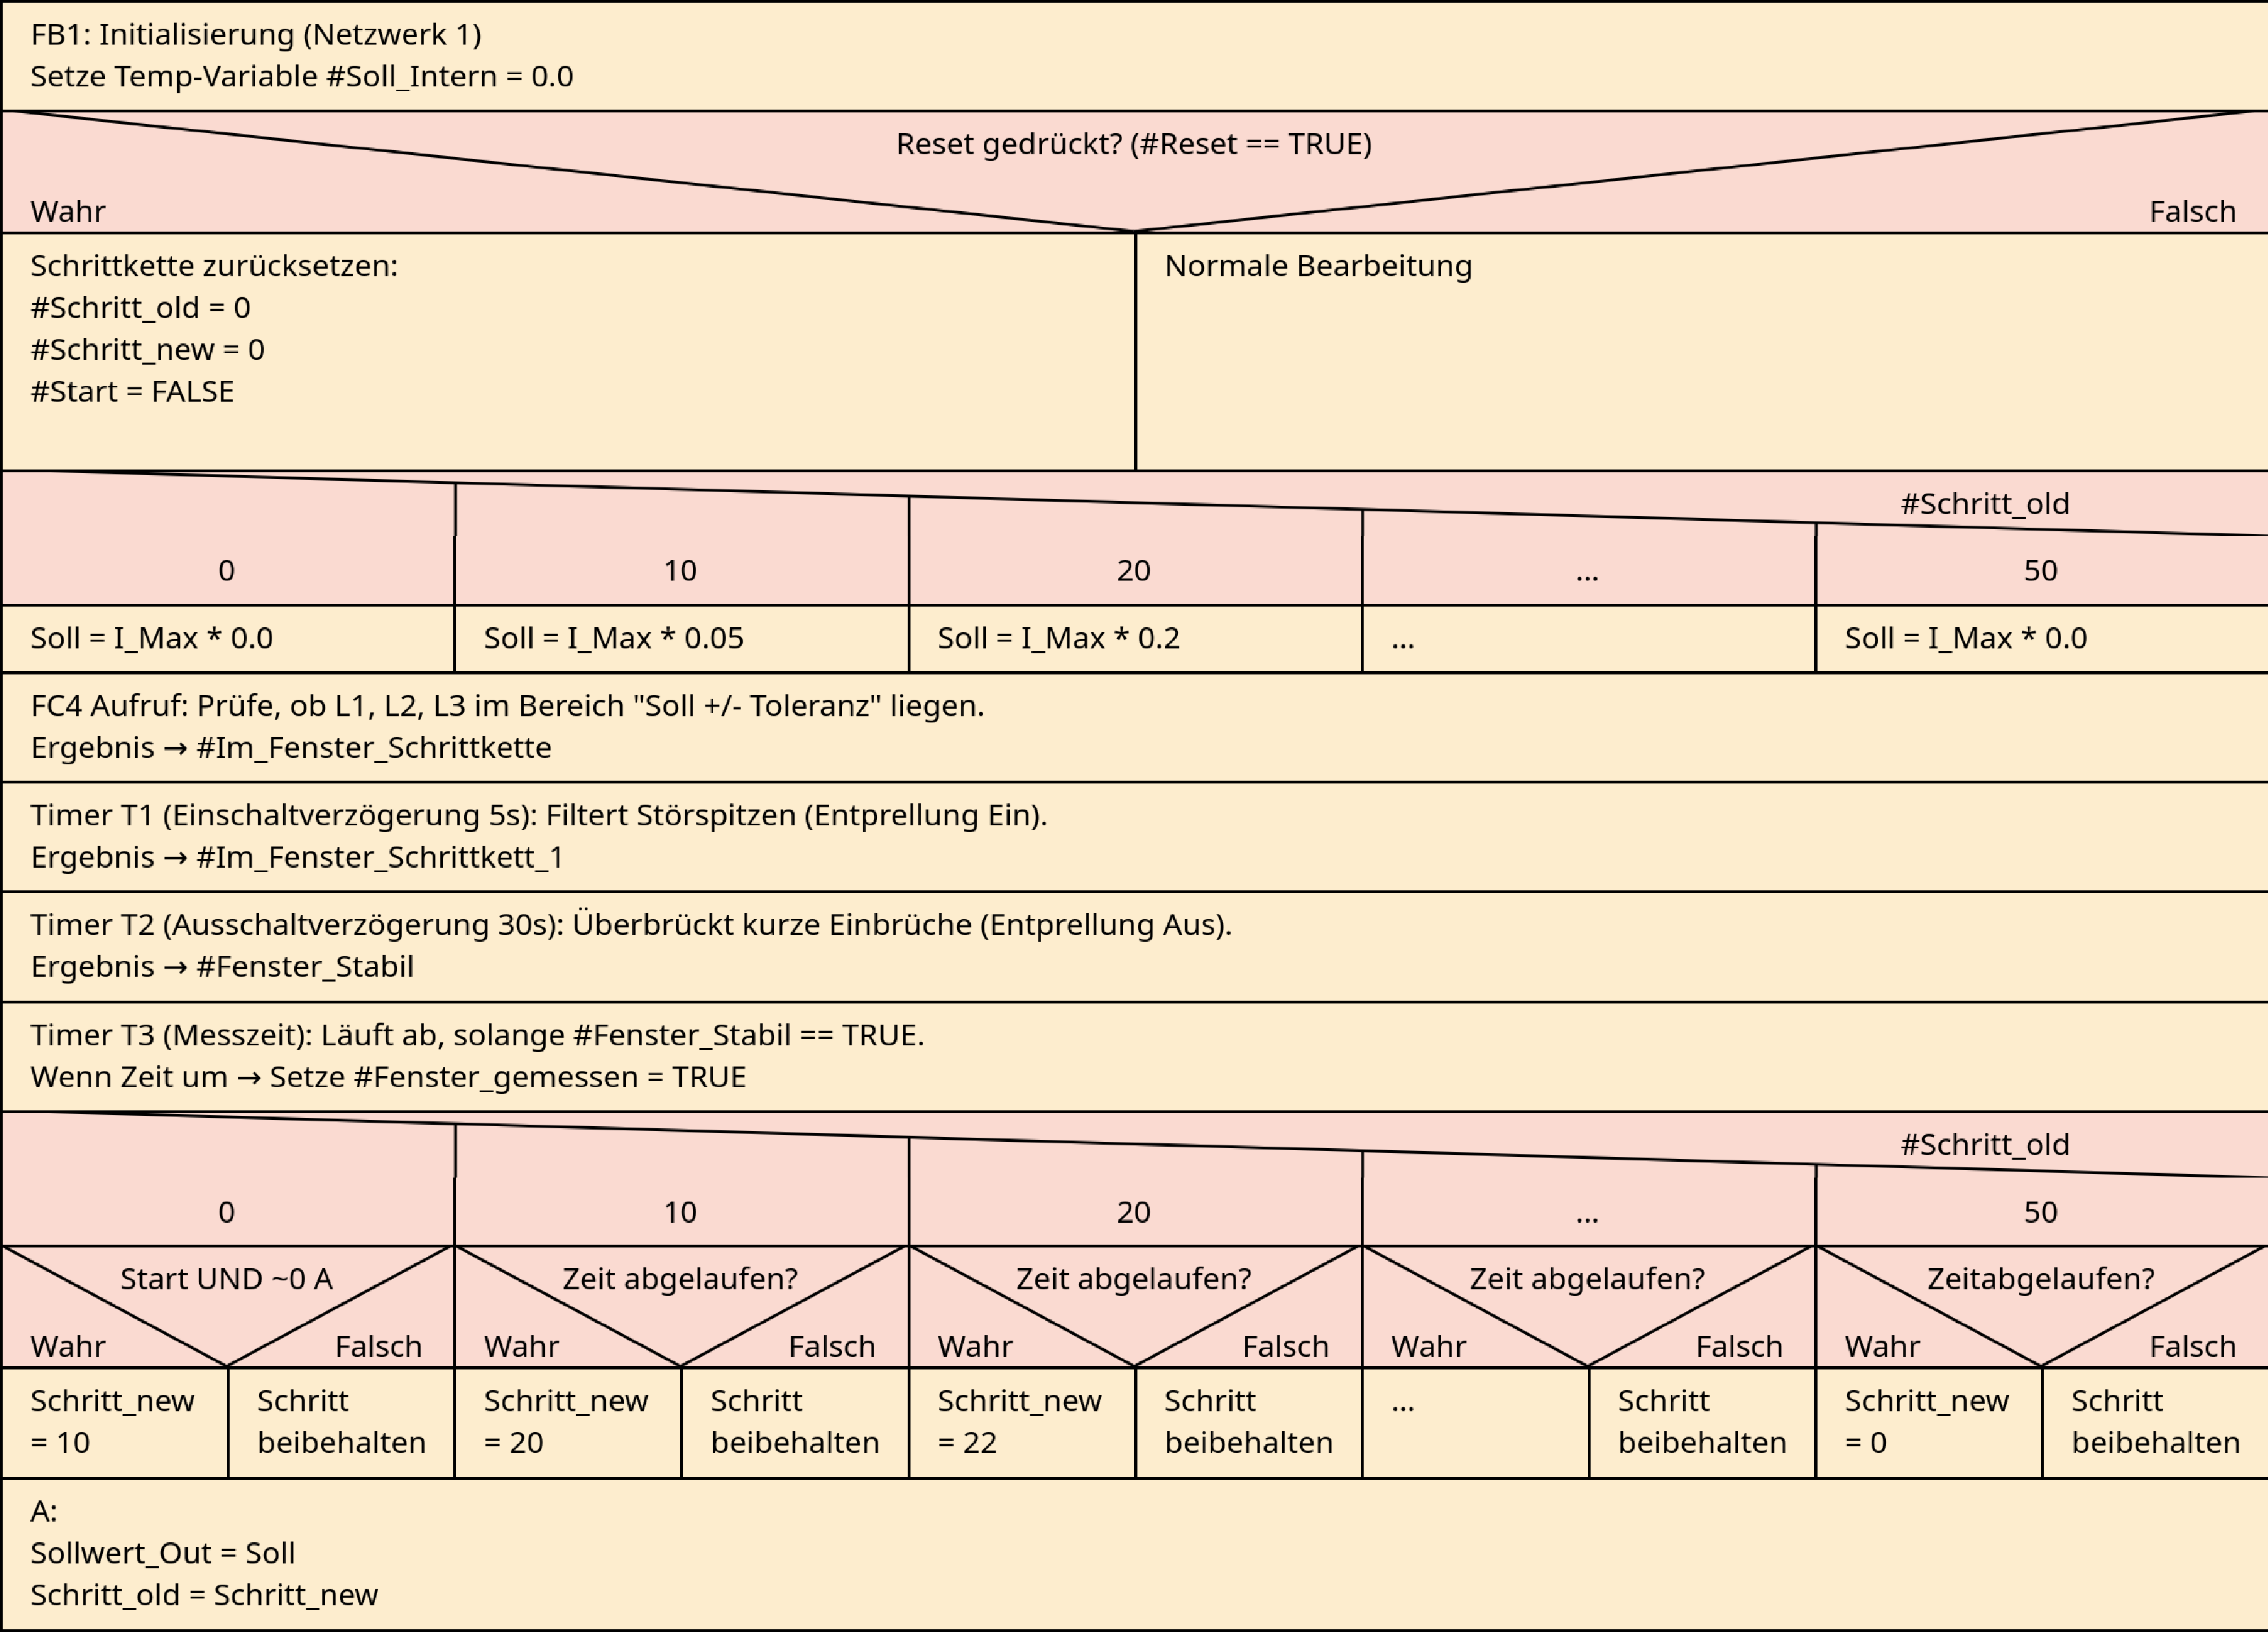
\includepdf[pages=-, frame, scale=0.8, pagecommand={\subsubsection{Struktogramm FB1}}]{03_Ressourcen/pdf/step7_programm/strukto_fb1.pdf}